% thesis.tex
% This is the main file, which calls up preamble.tex, frontmatter.tex, and thesis.bib as needed.

% Frontmatter shortcuts; note the extra space at the end, which is unfortunately necessary:
\newcommand\myname{Marcello Alves de Sales Junior }
\newcommand\mytitle{Persisting Collected Sensor Network Data: A New Approach Based on Schema-less Document-Oriented Databases }
\newcommand\thismonth{December }
\newcommand\thisyear{2009 }

% Shortcuts (add your own...):
\newcommand{\N}{\mathbb{N}}
\newcommand{\Z}{\mathbb{Z}}
\newcommand{\Q}{\mathbb{Q}}
\newcommand{\R}{\mathbb{R}}
\newcommand{\C}{\mathbb{C}}
\newcommand{\doubleS}{\mathbb{S}}
\newcommand{\vnorm}[1]{\left\|#1\right\|}
\newcommand{\degree}{\ensuremath{^\circ}}
% One of the following two has to be commented out:
%% draftpreamble.tex, to be used with thesis.tex
% This contains the TeX definitions for layout, style, etc., useful for the *draft* of your thesis.
% For the final version of your thesis, use preamble.tex

%%%%% TeX class and packages

\documentclass[12pt,oneside]{book}

\usepackage{amsthm,amsmath,amssymb,amsfonts,latexsym,graphicx,enumerate,setspace}
%\usepackage{color}                       % For creating colored text and background
%\usepackage{hyperref}                 % For creating hyperlinks in cross references
% other possibly useful packages: textcomp,mathrsfs,amscd,epsfig,euscript,cancel

%%%%% Layout

\voffset=-.8in 
\oddsidemargin=0in
\evensidemargin=0in
\textwidth=6.5in
\textheight=9in

\pagestyle{plain}

%%%%% Style of theorems, definitions, examples, equations, etc.

\theoremstyle{plain} % Heading is bold, text italic.
\newtheorem{theorem}{Theorem}[chapter]
\newtheorem{lemma}[theorem]{Lemma}
\newtheorem{proposition}[theorem]{Proposition}
\newtheorem{corollary}[theorem]{Corollary}
\newtheorem{conjecture}{Conjecture}[chapter]

\theoremstyle{definition}  % Heading is bold, text is roman
\newtheorem{definition}{Definition}[chapter]
\newtheorem{example}{Example}[chapter]

\theoremstyle{remark}  % Heading is italic, text is roman
\newtheorem*{remark}{Remark}
\newtheorem*{note}{Note}
\newtheorem{claim}{Claim}[chapter]

%%%%% Appendix style

\renewcommand\appendix[1]{
\chapter*{#1}
\addcontentsline{toc}{chapter}{#1}
}

%%%%% Comment command, useful for editing

\newcommand\comment[1]{{\sc Comment:} {\bf #1}}

%%%%% Draft title page

\begin{document}

\thispagestyle{empty}

\[ \]
\vspace{1in}

\begin{center}
{\Large \bf \mytitle}

\vspace{1.5in}

\myname

\vspace{1.5in}

Version of \today

\end{center}

\tableofcontents 
  % eco-friendly draft version
% preamble.tex, to be used with thesis.tex
% This contains the TeX definitions for layout, style, etc., as well as the first few pages of your thesis: title page, copyright page, approval page, abstract, acknowledgments, tables of contents, tables, and figures.
% The layout commands should give the correct margins according to the graduate division's guidelines

%%%%% TeX class and packages

\documentclass[12pt,oneside]{sfsuthesis}
\usepackage{amsthm,amsmath,amssymb,amsfonts,latexsym,graphicx,enumerate,setspace,verbatim,makeidx,subfigure, multirow, url, soul}
\usepackage[subfigure]{tocloft}
\usepackage{color}                       % For creating colored text and background
%\usepackage{hyperref}                 % For creating hyperlinks in cross
%references
% other possibly useful packages: textcomp,mathrsfs,amscd,epsfig,euscript,cancel

%%%%% Layout
% These numbers might depend on your printer. Check the margins and compare them to the Graduate Division's
% guidelines. If there's something off, try playing with the numbers...
%
% For chapters:
%     Must have a minimum of 1.5in margin on left and 1in on all other sides.  Where there are page numbers
%     (whether on top or bottom), must have one additional inch between the page number and the text, for a
%     total of 2in between the edge of the paper and the text.
% For frontmatter pages:
%     The same margin numbers generally work, except for the Title Page, so you will notice that we use
%     some numbers for \textheight and \footskip right here, and then change them below, right after
%     generating the Title Page.

\hoffset=.5in 
\oddsidemargin=0in
\evensidemargin=0in
\topmargin=0.1in 
\headheight=0in
\headsep=1in
\footskip=.8in
\textwidth=5.9in
\textheight=7in

\setcounter{secnumdepth}{3}
\setcounter{tocdepth}{3}

\pagestyle{plain}

\doublespacing

%%%%% Style of theorems, definitions, examples, equations, etc.

\theoremstyle{plain} % Heading is bold, text italic.
\newtheorem{theorem}{Theorem}[chapter]
\newtheorem{lemma}[theorem]{Lemma}
\newtheorem{proposition}[theorem]{Proposition}
\newtheorem{corollary}[theorem]{Corollary}
\newtheorem{conjecture}{Conjecture}[chapter]

\theoremstyle{definition}  % Heading is bold, text is roman
\newtheorem{definition}{Definition}[chapter]
\newtheorem{example}{Example}[chapter]

\theoremstyle{remark}  % Heading is italic, text is roman
\newtheorem*{remark}{Remark}
\newtheorem*{note}{Note}
\newtheorem{claim}{Claim}[chapter]

%%%%% Appendix style

\renewcommand\appendix[1]{
\chapter*{#1}
\addcontentsline{toc}{chapter}{#1}
}

%%%%% Source-Code listings

\usepackage{courier}
\usepackage{color}
\usepackage{xcolor}
\usepackage{listings}

\lstset{commentstyle=\tiny,captionpos=t,tabsize=2,frame=lines,keywordstyle=\color{blue}\tiny,commentstyle=\color{gray}\tiny,stringstyle=\color{red}\tiny,numbers=left,numberstyle=\tiny,breaklines=true,showstringspaces=false,basicstyle=\tiny,emph={label}}

%\definecolor{darkgreen}{named}{green}
%\definecolor{darkblue}{named}{blue}
%\definecolor{darkred}{named}{red}
%\definecolor{grau}{named}{gray}
%\let\Righttorque\relax
%\lstset{
%commentstyle=\itshape\color{darkgreen},
%keywordstyle=\bfseries\color{darkblue},
%stringstyle=\color{darkred},
%extendedchars=true,
%basicstyle=\scriptsize\ttfamily,
%basicstyle=\tiny\ttfamily,
%tabsize=2,
% keywordstyle=\textbf,
%commentstyle=\color{grau},
% stringstyle=\textit,
%numbers=left,
%numberstyle=\tiny,
% für schönen Zeilenumbruch
%breakautoindent = true,
%breakindent = 2em,
%breaklines = true,
%postbreak = ,
%prebreak = \raisebox{-.8ex}[0ex][0ex]{\ensuremath{\lrcorner}},
%prebreak = \raisebox{-.8ex}[0ex][0ex]{\Righttorque},
%showspaces=false, % Keine Leerzeichensymbole
%showtabs=false, % Keine Tabsymbole
%showstringspaces=false,% Leerzeichen in Strings
%}

\usepackage{caption}
\DeclareCaptionFont{white}{\color{white}}
\DeclareCaptionFormat{listing}{\colorbox{gray}{\parbox{\textwidth}{#1#2#3}}}
\captionsetup[lstlisting]{format=listing,labelfont=white,textfont=white}

%% Use fancy chapter headers, with Jos Dingjan's modifications,
%% plus my own tweaks. This style is not part of teTeX,
%% so we are using a local (and renamed) copy.
\usepackage[Lenny]{fncychap}

%Hifens
\usepackage[latin1]{inputenc}
\usepackage[USenglish]{babel}

%Harvard citation style
\usepackage{natbib}
%enhanced items
% http://dante.ctan.org/tex-archive/macros/latex/contrib/enumitem/enumitem.pdf
\usepackage{enumitem}

\begin{document}

\pagenumbering{roman}
\thispagestyle{empty}

\[ \]
\vspace{-1.8in}

\begin{center}
{\mytitle}

\vspace{1.4in}

\singlespace{A thesis presented to the faculty of\\
San Francisco State University\\
In partial fulfillment of\\
The requirements for\\ The degree}

\vspace{.5in}

\singlespace{Master of Science\\ In\\ Computer Science}

\vspace*{\fill}

{by \\[12pt] 
\myname \\[12pt]
San Francisco, California\\[12pt]
\thismonth
\thisyear}
\end{center}

\newpage
\thispagestyle{empty}

$\mbox{}$
\vspace{3in}
\begin{center}
\singlespace{
    Copyright \copyright{} \thisyear by \myname

    \bigskip

    All rights reserved. No part of the material protected by this
    copyright notice may be reproduced or utilized in any form or by any
    means, electronic or mechanical, including photocopying, recording or
    by any information storage and retrieval system, without the prior
    permission of the author.
}
\end{center}

\newpage
\thispagestyle{empty}
\[ \]
\vspace{-1.8in}
\begin{center}
{CERTIFICATION OF APPROVAL}
\end{center}
\vspace{.5in}
\begin{quote}
I certify that I have read {\it \mytitle} by \myname, and that in my opinion
this work meets the criteria for approving a thesis submitted in partial
fulfillment of the requirements for the degree: Master of Science in Computer
Science at San Francisco State University.
\end{quote}

\vspace{1.5in}

\hspace*{\fill}\parbox{3.5in}{
\singlespace{

\hrule{\hspace{3.5in}} \\ 
Prof. Arno Puder, Ph.D.\\
Professor of Computer Science\\
\vspace{1in}
\hrule{\hspace{3.5in}} \\
Prof. Marguerite C. Murphy, Ph.D.\\
Professor of Computer Science

}
}

\newpage
\thispagestyle{empty}
\[ \]
\vspace{-1.8in}
\begin{center}
{\mytitle} \\

\vspace{.5in}

\singlespace{
\myname \\
San Francisco, California \\  
\thisyear \\
}
\end{center}

\vspace{.5in}

%\doublespacing{\noindent
\onehalfspacing{\noindent      
Sensor Networks are becoming more and more important to different science
communities bacause of what they produce: the raw data for different studies.
In order to make use the collected data, researchers may have to dissect the
characteristics of the sensor network in question, regarding different
properties such as the purpose and location of the observed data, as well as
how the data is described. For this reason, this work proposes a set of data
persistence taxonomies based on the state of the art, which can be used to
classify the properties of the produced raw data. In order to evaluate the
proposed taxonomies, this work designs and implements a data persistence
component for NetBEAMS, our case study of modular sensor network infrastructure
developed to improve the operation of the SF-BEAMS environmental sensor
network. In this way, based on empirical analysis regarding proposed
taxonomies for the case study, this work selected mongoDB, a schema-less
document-oriented database instead of the traditional use of relational
databases. As a result based on the experiments conducted, this work suggests
that use of Key-Value Pair datasents in orde tor provide External of
Data-Centric approach. Therefore, the use of a solution of the help decreasing
the complexity related to the data persistence layer for sensor networks with
external or data-centric storage mechanism, and whose purpose is data
archival. Finally, this work proposes different future works such a
data-centric approach using Databa se Shards to store te collected data and Map
Reduce to execute parallel queries over the shards.} \vspace*{\fill}
 
\hspace*{\fill}

\noindent
I certify that the Abstract is a correct representation of the content of this thesis.

\vspace{.5in} 

\hrule{\hspace{3.75in}} \\[-10pt]
Chair, Thesis Committee 
\hspace{2.5in}
Date
\doublespacing
\newpage
\[ \]
\vspace{-1.8in}
\begin{center}{ACKNOWLEDGMENTS}\end{center}

\vspace{.5in}
\begin{quote}
\noindent
Acknowledgments
\end{quote}

\renewcommand{\contentsname}{\vspace{-1.7in} \begin{center} \normalsize \rm TABLE OF CONTENTS \end{center}}
\renewcommand{\listfigurename}{\vspace{-1.7in} \begin{center} \normalsize \rm LIST OF FIGURES \end{center}}
\renewcommand{\listtablename}{\vspace{-1.7in} \begin{center} \normalsize \rm LIST OF TABLES \end{center}}
\renewcommand{\cftchapfont}{\normalfont}
\renewcommand{\cftchappagefont}{\normalfont}
\renewcommand{\cftchapleader}{\cftdotfill{\cftdotsep}} % formatting commands for table of contents
\renewcommand{\cftsecfont}{\normalfont}
\renewcommand{\cftsecpagefont}{\normalfont}
\renewcommand{\cftsecleader}{\cftdotfill{\cftdotsep}}

\newpage \tableofcontents 
\newpage \listoftables % comment out if you don't use tables
\newpage \listoffigures % comment out if you don't use figures

\newpage
\pagestyle{myheadings}
\pagenumbering{arabic} 
\setcounter{page}{1}
   % final version, formatted according to the Graduate
% Division's guidelines

% Main body of work:

% main.tex, to be used with thesis.tex
% This contains the main work of your thesis.


%\bibliography{thesis}  % uses the references stored in Chapter1Radar.bib

\chapter{Introduction}

Sensor networks are commonly used in different areas for different purposes
such as scientific measurements and general population use
\cite{snintro01} \cite{snintro02}. In the scientific community, they serve as
tools to monitor the state of the environment by storing samples of data in specific 
periods of time. For instance, the NASA Jet Propulsion Laboratory uses the 
Volcano SensorWeb \cite{snex02}, a sensor network which aims to collect data
from specific volcanoes in Alaska and South Pacific to be used with heuristics 
regarding dangerous activities. Similarly, the National Data Buoy Center, a
department of the National Oceanic and Atmospheric Administration (NOAA)
\cite{snex03}, provides online data from different buoys in different coast
shores around the world regarding water quality, temperature, tides, etc, what 
characterizes sensor network for environmental monitoring \cite{snex01}.
Therefore, sensor networks can be seen as a very important scientific research and 
commercial field with direct application and use of its produced data.

In order to provide access to the collected sensor data, different approaches
can be taken to interrogate sensor devices. In general, the query process can
take place on the network nodes themselves, as it is called in-network, or in 
a centralized data sink. The former is generally used when the data is
collected at the sensor node on its local storage, being shown by \cite{sn-storage01}
\cite{sn-storage03} \cite{sn-storage04} that this strategy helps mitigating energy
consumption. However, this strategy is used when data archival is not the
primary reason, given the limited resources on the sensor devices. For this
reason, the the latter strategy has been used when the collected data is
primarily archived in a centralized database system for later reuse
\cite{sn-storage02}.

When it comes to data model implementation, the relational data model
\cite{db01} is one of the most used approaches to represent data in sensor 
network databases in any of the query processing strategies, and in most cases 
with a modified version of the SQL language \cite{sn-db-newop01}
\cite{sn-db-newop02}. However, the design of the database system must be done
with prior knowledge of the sensor types when  choosing the relational data
model, as the database design must be normalized \cite{db02} for the entities
already identified for the system. For instance, the introduction of a new
sensor device might represent a potential change on the database structure by
seeking a new normalized version of the database structure. In addition to
challenges of maintaining the database schema normalized, the use of Data
Provenance approaches in sensor network data \cite{sn-provenance01} usually
addresses the problem related with the lineage of data  and its full history.
However, once the data model is in place to receive the collected data, one of
the most important non-functional requirements in sensor networks is
scalability of the persistence storage. Since an operational sensor network
can produce huge amounts of data, it must be able to cope with the increase
and data load during data gathering, and yet provide users the same
performance during data retrieval by using different strategies such a
data-centric storage \cite{sn-storage03}.

In summary, this dissertation discusses the solution of a centralized
data-centric persistence storage component for the NetBEAMS \cite{nb01}, Data
Sensor Platform (DSP), an open-source \cite{se01} implementation of a sensor
network that primarily focused on environmental data produced by NetBEAMS. 
Different challenges can be related to the DSP in the context of sensor 
networks: data model, data persistence organization and strategy, and user data
access and distribution. First, NetBEAMS needs to provide means to safely 
represent sensor devices' properties without the need of restructuring any 
existing data model, taking into account the use cases from the main users. 
For example, a marine biologist may query the the persistence storage regarding
the temperature of a specific geographic region at the San Francisco Bay at a 
given time frame. Second, since a sensor network may experiment grown in terms 
of number of sensors, and consequently the number of data produced, the
persistence  storage must be able to reasonably scale and be well structured
in terms of storage space with the least service interruption. For instance,
if the persistence storage is close to reach its storage capacity, what
should the network administrator do? Last, but not least, the means to access 
the data for reuse is the most important features of the system, taking into 
account the different data formats used by the main users of the system. How 
to export specific collected data to a spreadsheet or archive files to be 
published or shared with other users? For these, and many other reasons, the 
persistence storage problem addressed by this work can be seen as a very 
challenging experience to solve.

In view of the fact that the persistence storage of a sensor network imposes
many different challenges, and taking into account the case study NetBEAMS, this
work's main strategy focused analyzing the different specifications of data
persistence in the literature in order to find new types of mechanisms to
provide data persistence for sensor network data. In this way, the kernel of
this dissertation is focused on providing solutions to the real-world problem
face by the Romberg Tiburon Center and its use of NetBEAMS. Furthermore,
the evaluation of different technologies is discussed in order to provide a
loosely-coupled component-based solution based on the infrastructure of the 
DSP Platform. For the reason of providing a 'lighter' data model, a subtype of
the Key-Value Pair \cite{kvp01} data model was chosen to easily capture the
description of any sensor device's properties, along with the use of time
series data models \cite{sn-provenance01} for time snapshots. In that way, data
modeling process does not represent a new refactoring each time a new sensor 
type is added or removed from the persistence system, giving users means to 
retrieve data accordingly. Similarly, in contemplation of scalability, this 
work proposes the use of an increasingly popular infrastructure technique called
Database Sharding \cite{dbshard01} \cite{dbshard02}, which takes the approach of
Data-Centric storage \cite{sn-storage03} on in-network query processing in a
centralized database system. In order to provide such mechanism, this work
evaluates the use of shard keys based on the geographic origin of the collected
data as cited to be one of the options when working with Provenance data in 
sensor networks \cite{sn-provenance01}. As a result, the data persistence system
component was conceived using the plug-and-play capability from the DSP 
platform without doing  any changes to the current DSP Platform, providing an
scalable solution that can adjust according to any data load increase. Finally,
the selected technology provides different data access mechanisms, which
directly addressed problems related to data access and Information Fusion 
\cite{sndp06}, providing export-import capabilities and visualization through
the availability of APIs written in different popular programming languages.

This dissertation report is organized as follows: the next chapter is an 
overview of the state of art on topics that supports the implementation of the
solution of this work, providing the necessary background foundation for the 
following chapters. Chapter 3 presents the design and architecture of the 
conceived persistence module, describing the requirements needed to be
addressed,  while Chapter 4 describes the implementation based on the design. 
The analysis and investigation of the implemented solution is shown through 
the analyzes of the experiment results on Chapter 5. Last, but not least, 
Chapter 6 presents the conclusions of this work, followed by the possible 
future works and recommendations presented on Chapter 7.
% main.tex, to be used with thesis.tex
% This contains the main work of your thesis.

%\bibliography{thesis}  % uses the references stored in Chapter1Radar.bib

\chapter{State of the Art}

Different aspects related to two major fields of Computer Science have
motivated to the inception of this work. In the perspective of Database
Systems and Distributed Systems, this work seeks a different approach for a
persisting collected data from sensor networks into a storage system that can
be seen as a cluster of distributed databases. Likewise, in the perspective of
Software Engineering, this work adds a major capability to an existing sensor 
network framework, meeting the requirements and interfaces. In general, this 
chapter gives the foundation based on the motivations for the inception of a 
different approach to persisting data using a different data model, covering 
topics that will be referred throughout the following other chapters.

This chapter will first give an overview on different related problems
described  in the literature that solved problems related to data modeling and 
representation in sensor networks. Then, it presents the design, architecture 
and implementation details of the DSP Platform, which is the bases for this 
dissertation. Finally, this chapter will briefly give a tutorial on advanced 
topics such as the differences between the KVP data model and the relational 
data model, as well as discussing about the approaches used on Database
Sharding.

\section{Sensor Networks}

Sensor Networks are specialized types of network systems comprised of network 
nodes with specific goals to observe and collect data. The following
subsections describe classes of characteristis of these types of sensor
networks, with applications on research, industrial or militery.

\subsection{Deployment and Mobility}

Each of the nodes can be deployed in a random way such as being dropped
from an airplane, or in a manual fashion at deliberately chosen geographical 
points \cite{sn-intro01}. Moreover, the deployment can be done as a one-time
event or an iterative way. 

However, nodes can be able to move around the deployed area or be static in
this place. In the case of the degree of the former behaviour, a sensor node
can move occasionally or continuously, being a result of an incidental 
side-effect or a desired property of the device, where they are an automotive
device or attached to another moving object. For this reason, \cite{sn-intro01} 
describes those types of mobility as active or passive.

\subsection{Device Size, Resources, Cost, Energy, Heterogeneity}

Such sensor nodes can be of different sizes, ranging from microscopically small
particles, small devices to bigger ones with a few feet cubic. In addition to
being limited in size, they are also limited in resources and computational
power, forcing their conception limited to have its energy stored in either
batteries or scavenged from solar cells \cite{sn-intro01}.

Since sensor devices range on size and capabilities, the cost for each of the
devices very from hundreds to thousands of dollars, depending on its
functionality, energy utilization, etc. For thie reason, \cite{sn-intro01}
explains that a sensor network may potentially contain similar sensor devices,
as they can contain dissimilar ones from each other, which characterizes the heterogeneity 
of a sensor network by the hardware capabilities such as GPS enabled or having
GSM  network connectivity.

\subsection{Communication Modality, Network Infrastructure, Coverage and
Connectivity}
\label{sec:sn-infrastructure}

Sensor nodes can communicate in different modalities such as radio, diffuse
light, inductive or sound, which may influence on the type of protocols used to
communicate among the nodes, where they can be said to be in an organized
infrastructure or as an ad hoc way \cite{sn-intro01}.

When it comes to the sensor network different organizational infrastructure,
they can differ in types of topology: single-hop, star, networked stars, tree
and graph, where each of them may affect the characteristics of the network as it 
may also influence on data gathering and routing mechanisms. While in a
single-hop sensor network there are only two levels of sensor connectivity, the
tree, graph or networked stars networks uses communications among the network
hosts for data communication.

Last, but not least, sensor networks may be influenced its coverage designed in
its purpose, its size in terms of number of nodes and its relating lifetime. As
sensors are deployed in different areas, they can be distributed in a sparse or
dense way, yet providing necessary coverage for the environment. However, 
considering that sensor devices are very likely to constant failures, projects 
have provided redundant nodes \cite{sn-intro01}. This degree of coverage also 
influences on the connectivity of the sensor nodes, where they can be
considered connected when a connection is available at all times. On the other
hand, nodes can communicate with other nodes in an intermittent way or sporadic
way. In the former, the sensor node is partitioned, while in the latter the
nodes are isolated most of the time and communicates at certain moments in
time.

\subsection{Network Size, Lifetime and Quality-Of-Service}

Similar to the degree of coverage of the sensor network is the number of
sensor nodes deployed in the network, where they can be in the order of
dozens, hundreds or even thousand of nodes \cite{sn-intro01}.

The application of the sensor network determines how long the sensor
network may be exist. For example, the lifetime of an environmental sensor
networks \cite{sn-ex01} may be not determined since its service serves in a
regular basis, whereas the lifetime of a sensor network to determine the number
of people in an event is limited to the event. 

Finally, the design of sensor networks can be related to the constraints
related to quality-of-service (QoS) such as real-time delivery within certain
period of time or robustness such as maintaining data alive even though there
a communication link is not available \cite{sn-intro02}.

\section{Data Persistence in Sensor Networks}

The most important purpose of a sensor network is related to its main product:
the use of the raw data. Data collection in sensor networks is directly
dependent on the specifications of the sensor network, its routing mechanisms
and the final destination of the produced data. In a nutshell,
\cite{sn-storage03} describes data as follows:

\begin{itemize}
  \item \textbf{low-level property} as the raw data collected from the
  sensor device; For example, the sea level as a number;
  \item \textbf{Observation or Event} as the processed data in format of the final
  observation. For instance, if the ocean is in its high tight or low tight.
\end{itemize}

\subsection{The Purpose of the Collected Data}
\label{sec:sn-data-purpose}

At first glance, the raw data serves as the primary product of the sensor
network. However, the first consideration that must take place is regarding the
purpose of the collected data, as \cite{sn-provenance01} explains
differentiates between two main use of the sensor data:

\begin{itemize}
  \item \textbf{Real-time Data Stream}, as the generated data from the sensor is
  actually not transmitted, but extracted from the device as it is requested.
  The data is still in its natural format specified by the sensor manufacturer;
  \item \textbf{Archival Data}, as the collected data have historical value or will
  be use by other applications at a future time. 
\end{itemize}

While real-time data stream are used and can potentially be discarded, the
archival data needs to be stored in a secondary memory. Nonetheless, given the
nature of the sensor device specification, the low-level data produced
by a given sensor device might not contain necessary information regarding the
identity of the data itself. The use of Data Provenance techniques is described
by \cite{sn-provenance01} as an important step to provide the collected data 
specific metadata regarding its location and lineage.

Under these circumstances, the collected data needs first to face its jorney
starting from its transmission from its producing device to the specified data 
sink as specified by \cite{sn-storage01} \cite{sn-storage02} \cite{sn-storage03}.

\subsubsection{Providing Identity to the Collected Sensor Data}

Most of sensor networks implementations use the collected data from the sensor
devices after they observe the environment. \cite{sn-provenance01} showed that
collected data used for archival purposes are usually missing important
features. First, the device's sampling are usually in raw format or without
obvious names. In order to provide search over the collected sensor data, the
data needs first to be described and indexed, and this process can be related
to Data Provenance \cite{db-provenance}. 

An example of Data Provenance application is the use of aggregation of data
over time to estimate the changing effects of the weather in a given region.
For this reason, the collected data needs descriptions or annotations that can
give enough information to track changes, that is, the history of how and when
a given data has changed. The following should be the foundation of a
provenance-aware collected data according to \cite{sn-provenance01}:

\begin{itemize}
  \item each low-level observation as it describes the actual data;
  \item the location where the collected data was generated;
  \item the time when the data was collected.
\end{itemize}

\subsection{Storage Location for Collected Data}
\label{sec:sn-storage-locations}

Given that collected data can be used for different purposes as described in
section \ref{sec:sn-data-purpose}, the sensor node that produces the data is
responsible to send the raw data to a specified data storage destination. Upon
producing data, a sensor network node is specified to deal with the produced
data, where in most cases, \cite{sn-storage03} described that depending on the
sensor network infrastructure (see section \ref{sec:sn-infrastructure}),
different storage mechanisms are provided:

\begin{itemize}
  \item \textbf{External Storage}: the sensor device sends the produced data to
  another sensor node that contains an external storage. 
  \item \textbf{Local Storage}: as it is the case of real-time data stream, where data
  is allocated on the sensor device's main read-only memory.
\end{itemize}

It is clear that the data flows from the sensor node to another depending on
the specification of the network. On the whole, the sensor network
infrastructure dictates where the data will flow to, as described in section
\ref{sec:sn-infrastructure}. \cite{sn-storage02} sees a wireless sensor
networks as a many-to-one data gathering pattern, when its organization is
based on single-hop or star. On the other hand, when the data organization is
structured as a graph, tree, etc, the data flows from one intermediate sensor
node to another until it reaches its final storage node as described by
\cite{sn-storage01} \cite{sn-storage03}. 

Last, but not least, yet a different storage strategy can be used: Data-Centric
Storage. This strategy aims at clustering the collected data based on a given nature of the
data such as location. Regardless the data storage mechanism used, the query
processing will depend on the sensor network infrastructure and data location.

\subsection{Query Processing for Storage Locations}

Given the different locations where the collected data might be as described in
section \ref{sec:sn-storage-locations}, different query processing for the
collected sensor data can be used as described by \cite{sn-storage03}:

\begin{itemize}
  \item {In-Network Query Processing}: sensor nodes that provides real-time
  data stream usually replies to requests to properties. Likewise, when the
  data is used for archival purpose, the data can be located at a network node
  specialized in storing the neighbors collected data. In this way, when a
  query is issued to the sensor network, the query processor will
  collectively verify every storage node for the collected data.
  \item {Centralized Query Processing}: a main network sink receives the
  collected data from the peer nodes. In this case, the query processor queries
  the solo centralized node for the overall values of the participating sensor
  devices.
\end{itemize}

There are pros and cons related to both of the approaches of query processing,
which are also related to the infrastructure, sensor network nature and 
requirements. The main goal of the in-network query processing is to decrease
the amount of data transmitted from the sensor devices to the final data sink, as
sensor devices are usually limited by constraints such as energy utilization 
\cite{sn-storage03}. Along with this strategy, the literature describes
different proposals that aims at upgrading the Structured Query Language (SQL)
adding location-sensitive clauses to the language \cite{sn-db-newop01}
\cite{sn-db-newop02}. However, this main problem related to this approach is
that it may potentially flood all nodes with query messages \cite{sn-storage04}.

In order to mitigate the problems related flooded nodes in in-network query
processing, the use of a Data-Centric storage strategy has been shown to be a
proven alternative for the sake of energy consumption \cite{sn-storage03}
\cite{sn-storage01}. Its main goal is to classify the collected data based in a
specific property, say location or event, in order to be sent to specific
storage nodes that relates to the observation. As the main outcome of this
strategy is to create network partitioning strategy, the query processor would
hit specific sensor nodes with the needed data, and therefore, would
decrease the load and maximize the capacity on the actual sensor devices.

A centralized network query processing processes data in a network node
specified as the network sink. The network sink usually is a network
node with a database server with the collection of data delivered by
all the sensor devices from the network. As a consequence of this
many-to-one communication strategy \cite{sn-storage02}, the query process does
not affect any of the sensor nodes in the network and, thus, maximizes the
sensor device utilization. Moreover, the use of the data for historical
purposes is easier to manage and give access to the primary end users of the
data, following the process of data processing, compression, aggregation, etc
\cite{sn-db02}.

Although this approach seems to be convenient to the point of view of the
sensor nodes and used as the tradeoff between achieving capacity and energy
consumption, the centralized data collector suffers from the annavoiable
creation of a point of traffic concentration \cite{sn-storage02}, also referred
to as the phenomenon of congestion, or funneling effect \cite{sn-storage04}.
For this reason, simple distributed system techniques such as the use of
master-slave or data replication can be used to decrease the overhead.

\section{SF-BEAMS: a Marine Sensor Network for Water Quality Monitoring}

The San Francisco Bay Environmental Assessment and Monitoring Station,
or SF-BEAMS, is a marine sensor network operated by the Romberg Tiburon Center
(RTC). This section details the SF-BEAMS sensor network located at
the Tiburon Island, California, and then presents the details of NetBEAMS, as
it is part of the case study of this work.

\subsection{The SF-BEAMS Infrastructure}

The RTC's main focuses are in the study of complex marine and estuarine
environments using the SF-BEAMS sensors deployed offshore of its pier located
on the banks of the San Francisco Bay at the Tiburon Island, California. In
this way, the project is responsible for providing data for water quality
monitoring, as well as weather and surface conditions. 

In general, the SF-BEAMS network infrastructure contains heterogeneous wired and
wireless devices standing on pilons docked in the pier, where each of them is
responsible for observing different conditions of the area, as well as having
its own mechanisms for internal storage for the collected data. In this way,
data can be directly transferred to the labs via ethernet cables or collected
manually download by a staff's laptop computer. Figure \ref{fig:sf-beams}
shows a picture taken from the SF-BEAMS web-cam placed in-site.

\begin{figure}
  \centering
    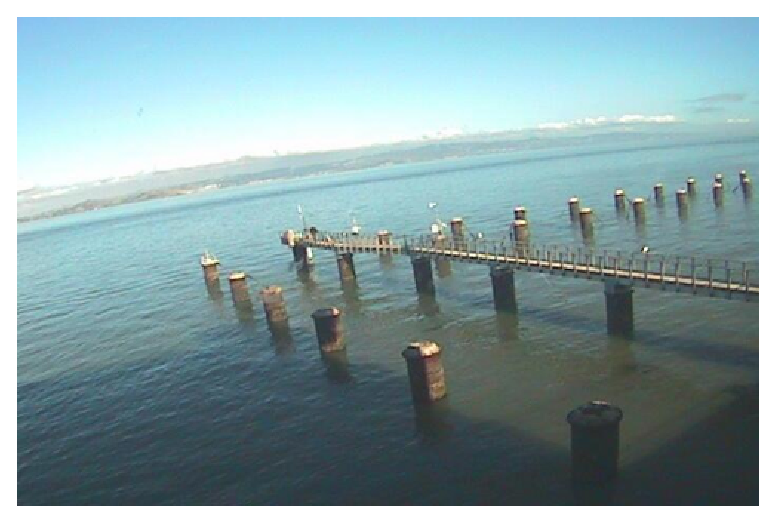
\includegraphics{../diagrams/cam_image-oct15}
  \caption{Picture of the SF-BEAMS Network, at the RTC pier. Tiburon, CA.}
  \label{fig:sf-beams}
\end{figure}

\subsection{SF-BEAMS produced data and collection process}
\label{sec:sfbeams}

As described in section \ref{sec:sn-infrastructure}, sensor devices generates
its observed data based on properties of measurements defined by its
manufacturer. SF-BEAMS is a single-hop star sensor network containing
different instances of sensors, including the "YSI 6600 ESD V2", as seen on
figure \ref{fig:ysi-device}, which is a powerful water quality monitoring
device that produces around 52 bytes (13x4 Bytes) on a single real-time data
stream as shown on table \ref{tab:ysi-data-stream}.

\begin{figure}
  \centering
  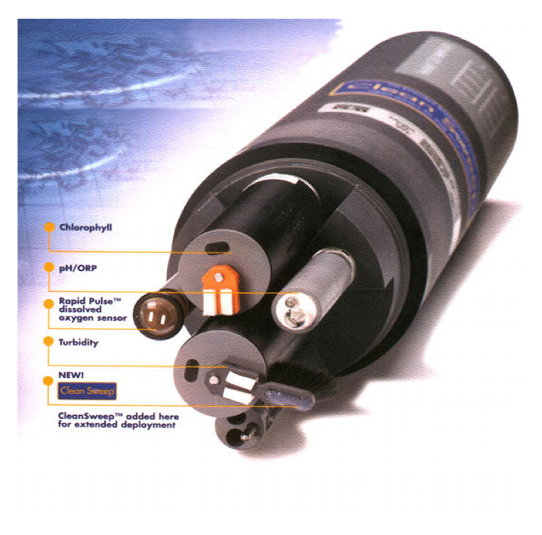
\includegraphics{../diagrams/ysi-device}
  \caption{Picture of the case study sonde device: YSI 6600 ESD V2}
  \label{fig:ysi-device}
\end{figure}

\begin{table}
    \caption{YSI Data Stream}
    \begin{center}
        \begin{tabular}{lr}
  12.20    192    179 5588.40   0.09   0.084   0.059  7.98   -79.6   99.5  8.83 
  0.4     8.7
        \end{tabular}
    \end{center}
    \label{tab:ysi-data-stream}
\end{table}

In order to have access to the observed data, the network staff downloads
the data using one of the device's connection such as the RS-232 serial
connector \cite{rs232}. Then, the data is transferred to the RTC labs for
archival, where it is described, indexed and distributed to its main users.
According to its staff members, in May 2009 the infrastructure of the SF-BEAMS
included the following was organized as follows:

\begin{itemize}
  \item 5 YSI sondes in operation at the RTC site Pier in Tiburon Island, San
  Francisco Bay;
  \item Each YSI sonde produces 52 Bytes for each its observations;
  \item The sampling frequency rate could be configured in ranges of 1, 6 or
  15 minutes, depending on the staff's speficiation. 
\end{itemize}

Considering the infrastructure previously described, the size of the data
produced by the YSI sonde sensors at the RTC pier can estimated by its
measurement frequency as follows:

\begin{table}
    \label{tab:ysi-data-distribution}
    \caption{Amount of data produced by the RTC's YSI sondes}
        \begin{center}
        \begin{tabular}{|c|c|c|c|c|c|c|}\hline 
        \textbf{YSIs} & \textbf{Rate} & \textbf{Hourly} & \textbf{Daily} &
        \textbf{Weeky} & \textbf{Monthly} & \textbf{Yearly}\\\hline 
        1 & 1 min & 3.04 Kb & 73.12 Kb & 511.87 Kb & 1.99 Mb & 23.99 Mb\\\hline 
        5 & 6 min & 15.23 Kb & 365.62 Kb & 2.5 Mb & 9.99 Mb & 119.97 Mb\\\hline 
        1 & 15 min & 0.5 Kb & 12.18 Kb & 85.31 Kb & 341.25 Kb & 3.99 Mb\\\hline 
        5 & 1 min & 2.54 Kb & 60.93 Kb & 426.56 Kb & 1.67 Mb & 19.99 Mb\\\hline
        1 & 6 min & 0.2 Kb & 4.87 Kb & 34.12 Kb & 136.5 Kb & 1.6 Mb\\\hline 
        5 & 15 min & 1.0 Kb & 24.37 Kb & 170.62 Kb & 682.5 Kb & 7.99 Mb\\\hline
        \end{tabular}
        \end{center}
\end{table}

As it is shown, the data produced by this type of sensor runs in the order of
at most hundreds of Megabytes a year, what can be considered a very low data
storage requirement. Upon collecting the data from sensors, the RTC lab staff
use automation scripts written in Matlab to process, index and distribute the
raw data in different formats, including the OPeNDAP \ref{opendap}, a format
widely used in the research institutions that promotes easier data exchange
among them.

Although the execution of the RTC SF-BEAM sensor network produces its
execution, many operational challenges were faced by this type of
infrastructure, when it comes to the data utilization of wireless sensors that
are deployed in offshore conditions, \cite{netbeams2009} described the
operational challenges faced by the RTC staff and proposed NetBEAMS, a
component-based infrastructure that uses common-off-the-shelfs (COTS) embedded
systems and software to automate the process of data collection. Next section
describes how NetBEAMS is used to extract data from the SF-BEAMS sensor network.

\section{NetBEAMS: a Real-World Case Study on Environmental Sensor Network}

The Networked Bay Environmental Assessment and Monitoring System, or NetBEAMS, 
is a work-in-progress joint project proposed by the department of Computer
Science and the RTC at San Francisco State University. As described by
\cite{netbeams2009}, the solution can be used to automated the data gathering
process of the SF-BEAMS as described in section \ref{sec:sfbeams}. This
section fully details how NetBEAMS is executed in order to collect data from
SF-BEAMS, describing pertinent design and architectural details.

One of the motivations for the inception of NetBEAMS was the automation
of the data gathering and processing from the SF-BEAMS sondes without requiring
human intervention. Most importantly, the decrease with the costs of constant 
offshore site visits by boat, where biologists need manually collect the data
from the sensor devices in order to take them for further processing at the
lab. For this reason, the NetBEAMS research group proposed the use of the Data
Sensor Platform (DSP) \cite{netbeams2009}, as the second attempt to automate
the operation of SF-BEAMS.

This following sections details the DSP, its architecture and how data is
transported from the network nodes to the main network sink, the RTC labs.

\subsection{The Data Sensor Platform (DSP)}

The Data Sensor Platform, in short DSP Platform, is based on a micro-kernel
architecture developed on top of the Java modular framework called OSGi
\ref{osgi}. The platform represents the foundation of the execution of
NetBEAMS, since it is executed from an embedded hardware called Gumstix
\ref{gumstix} using a Linux operating system and on top of the Java Virtual
Machine (JVM). In order to transport data from sensors hosts to the network
sink, the use of a cellular connection is used to transport the collected data
from the senso devices using the HTTP Protocol, as described by
\cite{netbeams09}. Figure \ref{fig:sf-netbeams-node} shows the
architecture of the inhanced node designed by the NetBEAMS research group.

\begin{figure}
  \centering
  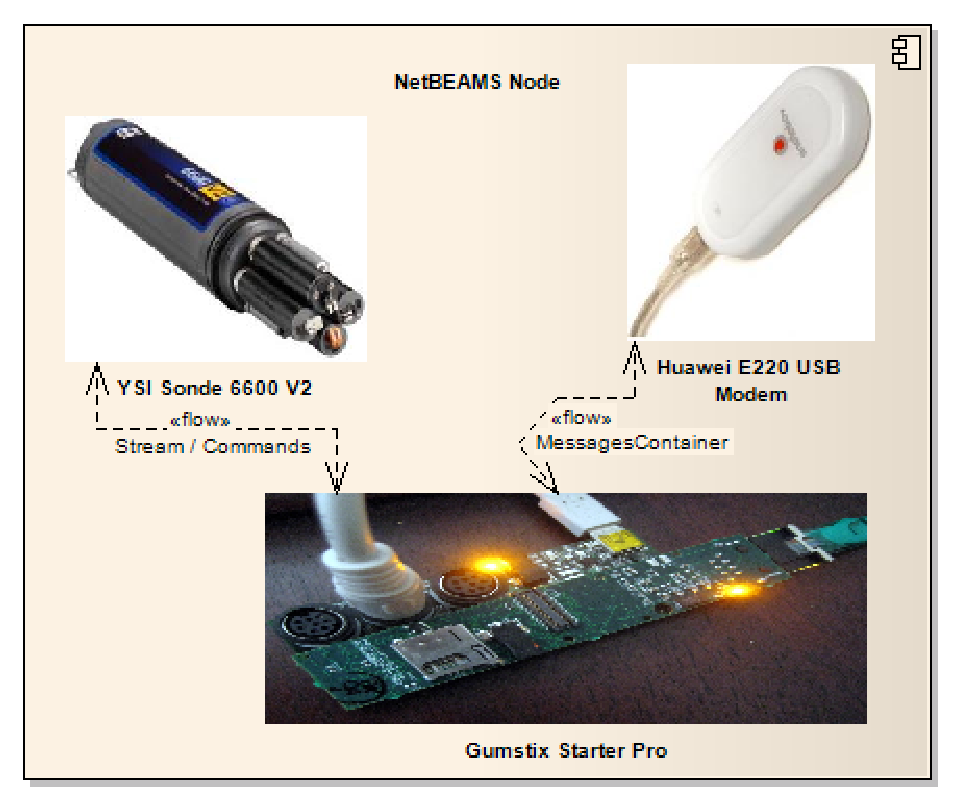
\includegraphics{../diagrams/DSP-Gateway-Node}
  \caption{The NetBEAMS Node enhancement with the Gumstix and the GSM Modem}
  \label{fig:sf-netbeams-node}
\end{figure}

The following list describes each of the devices in the NetBEAMS Node.

\begin{itemize}
  \item \textbf{YSI 6600EDS V2}: the YSI device is the regular sonde
  responsible for observing the environment. It is connected to the Gumstix
  embedded system, where the DSP is executed;
  \item \textbf{Gumstix console-vx}: it's a COTS ARM-based hardware that
  provides a computer-on-module environment for the development of small
  embedded systems. This is the main environment of data extraction and remote
  processing is accomplished. It runs a cross-compiled version of Linux Kernel
  2.6;
  \item \textbf{Huawei E220 USB Modem}: it is used to transfer the data from the
  Gumstix to the RTC Labs Data Center.
\end{itemize} 

The DSP runs inside of the embedded system Gumstix. The following sections
details its design and process for extracting data.

\subsection{The DSP System Design}

This section focus on the development of a Software Platform for the NetBEAMS Gateway Embedded System, or on the system developed in the Gumstix device. As shown on Image 2.4.1.1, the NetBEAMS Gateway Node is an embedded system that contains a set of layer found in any computer. However, each of the resources described from the system were customized for the NetBEAMS system. The main components of such system can be summarized as follows: 

    * Operating System: it uses a cross-compiled Gentoo Linux, which supports a wide variety of development tools, including the Java Virtual Machine (JVM), the underlying platform system;
    * Java Virtual Machine: it uses the JamVM, a ~200 KB version of the Sun Microsystems Java Virtual Machine, version 2.0;
    * OSGi Framework: it uses the Knopflerfish implementation of the OSGi 4.1 specification. More details in the following sections.
    * DSP Platform and other Bundles: The plug-and-play DSP Components are based on the OSGi bundles capabilities, which can reuse services registered in the OSGi framework.
% main.tex, to be used with thesis.tex
% This contains the main work of your thesis.

%\chapter*{Appendix A: Triangulations of Polytopes}
%\addcontentsline{toc}{chapter}{Appendix A: Triangulations of Polytopes}

\appendix{Appendix A: DSP Data Persistence OSGi Bundle}

This section includes the source-code for the DSP Data Persistence. Each
section details one single main artifact used on the development of the
component. However, only the main ones will be added into this document, while
the remainder can be downloaded directly from the Subversion repository.

The source code is located in the Subversion repository for the NetBEAMS
project. This is how it is structured:

%    DSP_HOME - http://code.google.com/p/netbeams/source/browse/ main
%    repository for evaluation.
%    - $PERSISTENCE = DSP_HOME/browse/branches/marcello/persistence/ = defines
%    the project home for the persistence component.
%    
%    - PERSISTENCE/versions/v2/apps/osgi-bundles/dsp/DSPDataPersistence =
%    defines the directory for the persistence bundle.

\section{OSGi Bundle Build}

This artifact defines the ANT build file.

\lstinputlisting[language=Ant,label=persistence-builder,caption=Build
system using Apache
ANT]{../../../../netbeams/versions/v2/apps/osgi-bundles/dsp/DSPDataPersistence/build.xml}

\section{DSP Data Persistence Service}

\lstinputlisting[language=Java,label=persistence-component,caption=DSP
Data Persistence
Component]{../../../../netbeams/versions/v2/apps/osgi-bundles/dsp/DSPDataPersistence/src/org/netbeams/dsp/persistence/controller/DSPDataPersistence.java}


% Bibliography (calls up the entries in thesis.bib if you run bibTeX):
\bibliographystyle{unsrt}
\addcontentsline{toc}{chapter}{Bibliography}
\singlespacing
\bibliography{thesis}

\end{document}
